\chapter{A lâmpada elétrica}
\label{sec:alampada}

Existem vários tipos de lâmpadas elétricas:
\begin{itemize}
\item Incandescente;
\item Fluorescente;
\item de Vapor de Sódio;
\item entre outras. % péssima ideia, não coloque isso no seu TCC
\end{itemize}

O símbolo elétrico utilizado para a lâmpada incandescente está
exposto na Figura \ref{fig:simbolo_lampada}.

\begin{figure}[!htb]
\centering
\begin{tikzpicture}
\draw (0,0) to[lamp] (2,0);
\end{tikzpicture}
\caption{Símbolo elétrico da lâmpada incandescente}
\label{fig:simbolo_lampada}
\end{figure}

O circuito elétrico ligando uma lâmpada geralmente se dá da
seguinte forma:

\begin{figure}[!htb]
\centering
\begin{tikzpicture}
\draw (0,0) to[sV] (0,2) to[closing switch] (2,2) to[lamp] (2,0) -- (0,0);
\end{tikzpicture}
\caption{Circuito elétrico da lâmpada}
\label{fig:circuito_lampada}
\end{figure}

A lâmpada incandescente, sendo ela representada eletricamente por
uma resistência, obedece à relação Volt-Apere da Equação \ref{eq:vri}.

\begin{equation}
\label{eq:vri}
V=R I
\end{equation}

Sendo representada graficamente de acordo com a Figura \ref{fig:vri}.

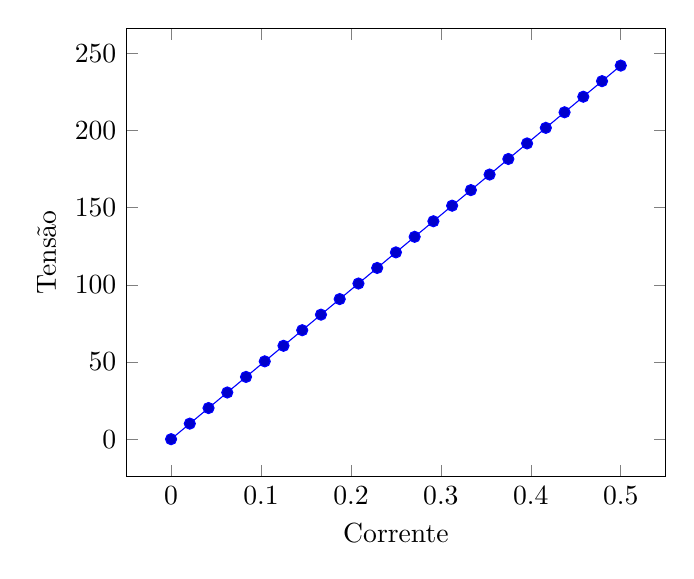
\begin{tikzpicture}
\label{fig:vri}
\centering
\begin{axis}[xlabel=Corrente,ylabel=Tensão]
\addplot+[domain=0:0.5] {484*x};
\end{axis}
\end{tikzpicture}
